\chapter{Evaluation and discussion}\label{results_discussion}

To protected PostgreSQL-process against infinite recursion, the execution stack is limited in size. The default in PostgreSQL 10.6 (\texttt{max\_stack\_depth}) is set to 2MB and can be manually increased. The maximum stack size is capped by the settings of the Operating System.\\
The available working memory (\texttt{work\_mem}) specifies how much memory can be consumed by in-memory operations like sorting or hashing. If the memory is exceeded, temporary results are stored on disk. Per default the working memory is set to 2MB. \cite[p. 512 ff.]{psql}

To fully exploit the capabilities of each implementation variant, the stack size is set to 7680kB (the limit of the OS) and working memory to 512MB. This way the recursive variant will not be terminated (too) early and the translation should be able to perform all computations in memory.

Using auto\_explain to track execution slows down by ca. 25\%.


\section{Original vs Translated Fibonacci Function}

\begin{figure}[h]
    \centering
    \includesvg{plots/fib_orig_vs_trans}
    \caption{Run time of fibonacci function in various versions.}
    \label{fig:fib_times}
\end{figure}
Runtimes vary greatly between the original recursive implementation, the automatic translation and a third, manually optimized fibonacci function\footnote{From \url{https://wiki.postgresql.org/wiki/Fibonacci_Numbers}, accessed: 15/12/2018}. To represent the wide variety the plots are drawed with logarithmic scales.

The original implementation is faster for very small inputs as it has less overhead then the translation. Additionally, the first two (fib(\$n-1) and fib(\$n-2)) calls are inlined. Anyway, the runtime of the original function grows very fast, so that $fib(30)$ already takes minutes. The translated function on the other hand is much faster. Where the original takes minutes, the translation is finished under 10ms. Even for fib(1000) the call returns after around 2 seconds. Yet, the translation cannot keep up with the manually optimized function. The same input here yields an result after a few milliseconds. But even here the runtime grows strongly as the inputs gets even larger. Yet, other limitations finally stop computing even larger fibonacci numbers: Somewhere between fib(600000) and fib(700000) the numeric datatype (which can represent numbers up to 131072 digits \cite[p. 124 f.]{psql}) fails with an overflow. That said, the manual optimized implementation is "as good as we can get".

The plot shows nicely how the automatic translation is magnitudes faster as the functional implemented original -- but the manually optimized implementation is again magnitudes faster. This affirms our initial claim, that our automatic translation gives you an great instant speed-up. Where the naive implementation gets slow, you can use the translation and the run-time drops from minutes to milliseconds. Where the translation runs for minutes, nothing else remains and you have to manually optimize the function. 

\subsection{Degree of recursion, DP}

\begin{figure}[h]
    \centering
    \includesvg{plots/branchN_dp}
    \caption{Comparision of UDF \texttt{branchN} (see \autoref{udfs:branchN}).}
    \label{fig:branchN}
\end{figure}

\subsection{Degree of recursion, DQ}

\begin{figure}[h]
    \centering
    \includesvg{plots/branchN_dq}
    \caption{Comparision of UDF \texttt{branchN} (see \autoref{udfs:branchN}).}
    \label{fig:branchN}
\end{figure}


\subsection{Varying number of arguments}

\begin{figure}[h]
    \centering
    \includesvg{plots/paramN_noopt}
    \caption{Run time of a same function (see \autoref{udfs:paramN}) with varying argument numbers. The translations are run using the generic template, without optimizations.}
    \label{fig:paramN}
\end{figure}

\autoref{fig:paramN} looks surprising. The original functions perform all equally and much better than the translations. Even more interstingly, the UDF with just one argument performs worst. This behaviour is surprising as we would guess that a simpler functions performs better in the translation because there is less data to manage and jonining tables is easier.\\
A first idea is, that the additional arguments give the functions more selective join predicates. Yet, this cannot be the case as the additional arguments of the used functions are just the arguments passed to the function, so the values are equal for all calls.\\
The reason for the big difference lays in the join order of the evaluation, as the query plan reveals. The function with one argument and n=200 makes first a nested loops anti join to join \texttt{evaluation} (rows=500, actual=68) with \texttt{callgraph} (rows=1, actual=201). The result (rows=1, actual=100) is joined with an hash join with \texttt{evaluation} (rows=500, actual=101).\\
The UDF with four arguments has flipped the order of the joins: First a hash join between \texttt{evaluation} (rows=940, actual=102) and \texttt{callgraph} (rows=100, actual=201) happens. The result (rows=1, actual=101) is joined with a nested loop anti-join with \texttt{evaluation} (rows=940, actual=69).

The problem is caused by the wrong guess about the number of rows returned from the scan of \texttt{callgraph}. The plans (see \autoref{plan:paramN}) are identical except for scenario-evaluation. During scenario-evaluation the CTE \texttt{e} (proxying \texttt{evaluation}) is joined with \texttt{callgraph} two times: Once for finding callsites of evaluated calls and once to check if the result is not yet calculated. The planner assumes that only a single row is returned using the filter \texttt{c.callsite\_id IN (1)}. But the UDF has only a single callsite, therefore the predicate is not selective at all.\\
The plan for the function with a single argument uses a \textit{nested loop anti join} to join the (supposed) single row from \texttt{callgraph} with \texttt{evaluation}. Nested Loop Joins are  a good choice when one table is small, otherwise a hash join performs better. The other plan uses first a hash join and than the nested loop join. As result, the nested loop join is executed on a smaller table which explains the better run-time. The plan from the UDF with one argument performs a nested loop join on tables with 68 and 201 rows, while in the other plan the inputs are sized 69 and 101 rows.

Now to the observation that the original performs better than the translation. This can be explained by the property, that the given function is linear recursive. No branching occurs and no memoization can be exploited. The overhead of the translation is significant is such a case: The evaluation-CTE adds in each step all the previous results to the new result. The number of rows is therefore $(0 + 1) + (1 + 1) + (2 + 1) + \dots + (n + 1) = \frac{n(n+1)}{2}$ and thus in $O(n^2)$. With the translation, we have made a linear function quadratically. Note that the results were obtained with optimizations disabled. So there is hope, as we see in the next section comparing optimizations to their originals.

\subsection{Optimizations}

\begin{figure}[h]
    \centering
    \includesvg{plots/paramN_opts}
    \caption{Comparision of UDF \texttt{param4} (see \autoref{udfs:paramN}) with varying optimizations.}
    \label{fig:paramN}
\end{figure}

% When limiting stack size to 100kb, param1_tr(320) is the first argument where it dies with "stack depth limit exceeded". As the function is nearly as simple as it gets, is seems to be valid to assume as lower bound that SQL will consume 1/3 kB per layer on the callstack. With default OS settings of max of 8MB on my machine, this means a maximum recursion depth of not more than roughly 25000 layers.  


\begin{figure}
    \centering
    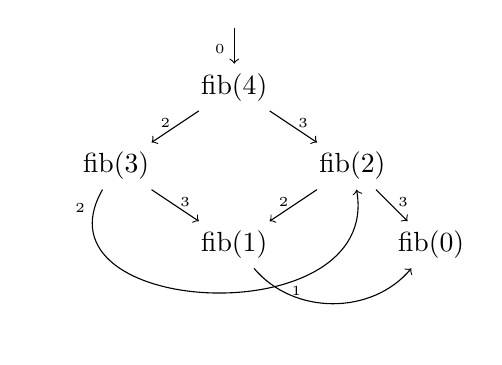
\begin{tikzpicture}
% nodes
\node (f4)     at (2.5, 2) {fib(4)};
    \node (f3) at (1, 1) {fib(3)};
        \node (f1) at (2.5, 0) {fib(1)};
    \node (f2) at (4, 1) {fib(2)};
        \node (f0) at (5, 0) {fib(0)};
% arrows
\draw[<-] (f4) -- node[pos=0.4, left, label distance=5mm]{\tiny{0}} +(0, 0.75);

\draw[->] (f4) -- node[pos=0.4, left, label distance=5mm]{\tiny{2}} (f3);
\draw[->] (f4) -- node[pos=0.4, right, label distance=5mm]{\tiny{3}} (f2);

    \draw[->, bend right=100, out=240, looseness=1.5] (f3) to node[pos=0.05, left, label distance=5mm]{\tiny{2}} (f2);
    \draw[->] (f3) -- node[pos=0.4, right, label distance=5mm]{\tiny{3}} (f1);
    \draw[->] (f2) -- node[pos=0.4, left, label distance=5mm]{\tiny{2}} (f1);
        \draw[->, bend right=50] (f1) to node[pos=0.2, right, label distance=5mm]{\tiny{1}} (f0);
    \draw[->] (f2) -- node[pos=0.4, right, label distance=5mm]{\tiny{3}} (f0);
\end{tikzpicture}
    \caption{Callgraph with memoization, The callstack-tree becomes a Directed Acyclic Graph (DAG). Each node represents an invocation and each outgoing edge a new callsite. Because of memoization, evaluation of equal invocations is performed only once, ie. they have the same descendants.}
    \label{fig:fib_callstack_memoization}
\end{figure}


\section{Advantages} Moimization, memory limitation, query planner
\section{Original vs. Translation}
\subsection{Number of recursive cases}
\subsection{Number of basecases}
\subsection{Number of parameters}
\subsection{Branching factor}

\section{Optimizations}
\subsection{Linear Recursion}
\subsection{Tail Recursive}
\subsection{Constant Parameters}

\section{Bottlenecks}